% =============================================================================
% P3A -- Privacidade 2: pôster (PT-BR), versão style2
% Estilo do pôster da P2A (_grupo/P2A/mainV3.tex): a0poster A1 retrato, marca da UnB,
% título em versalete verde, duas colunas com títulos azuis numerados, sem caixas.
% Figuras esperadas em out/: Fig1_PT.pdf, Fig2_PT.pdf, Fig4_PT.pdf (compiladas de figuras/).
% Marca da UnB: figuras/marca_unb.png. Conteúdo igual ao do pôster P3A_Privacidade2_Poster_PT.tex.
% =============================================================================
\documentclass[a1,portrait]{a0poster}
\usepackage[brazil]{babel}
\usepackage[utf8]{inputenc}
\usepackage[absolute]{textpos}
\usepackage{graphicx}
\usepackage{color}
\usepackage{xcolor}
\usepackage{amsmath,amssymb}
\usepackage{booktabs}

\definecolor{DarkBlue}{rgb}{0.1,0.1,0.5}
\definecolor{Red}{rgb}{0.9,0.0,0.1}
\definecolor{DarkGreen}{rgb}{0.10,0.50,0.10}

\let\Textsize\normalsize
\def\LHead#1{\noindent{\LARGE\color{DarkBlue} #1}\smallskip}
\def\Subhead#1{\noindent{\large\color{DarkBlue} #1}}
\newcommand{\quiteHuge}{\fontsize{55}{70}\selectfont}
\def\Title#1{\begin{center}\noindent{\quiteHuge\color{DarkGreen}#1}\end{center}}
\newcommand{\figcap}[1]{\par\vspace{0.2cm}{\centering\small #1\par}}

\TPGrid[40mm,40mm]{23}{12}

\parindent=0pt
\parskip=0.5\baselineskip

\begin{document}
\large

\begin{textblock}{23}(0,0)
\centering

\includegraphics[width=18cm]{figuras/marca_unb.png}
\end{textblock}

\begin{textblock}{23}(0,0.5)
\Title{\textsc{Privacidade no PMBOK 8: um domínio de desempenho proposto para a concentração Quem}}
\end{textblock}

\begin{textblock}{23}(0,1.1)
\begin{center}
  \parbox{0.8\textwidth}{
    \small
    \begin{center}
    \textbf{Autores:} Filipe Alves de Sousa, Emanuel Brandão de Galvão Correia, Ruben Isaac Dias da Silva e Carlos Eduardo da Silva Papa\\
    \textbf{Disciplina:} Gestão de Projetos de TI (GPTI) -- PPCA/CIC/UnB\\
    \textbf{Professores:} Dr. João Mello da Silva e Dr. Edison Ishikawa\\
    \textbf{Entrega:} P3A | \textbf{Código:} 3p2 / 3R31
    \end{center}
  }
\end{center}
\end{textblock}

% ------------------------------- COLUNA ESQUERDA ------------------------------
\begin{textblock}{11}(0,2.0)

\LHead{1. Problema e proposta}

O PMBOK 8 [13] menciona proteção de dados e privacidade, mas seus sete domínios e 40 processos não organizam o tratamento de dados pessoais como objeto próprio de gestão. Propomos \textbf{Privacidade} na concentração \textbf{Quem}, em diálogo com Partes Interessadas e Riscos.

\textbf{Pergunta-guia:} que efeitos o projeto produz sobre as pessoas cujos dados trata, e que evidências justificam suas decisões?

\vspace{0.3cm}
\LHead{2. Onde entra Privacidade}

\begin{figure}[h!]
\centering
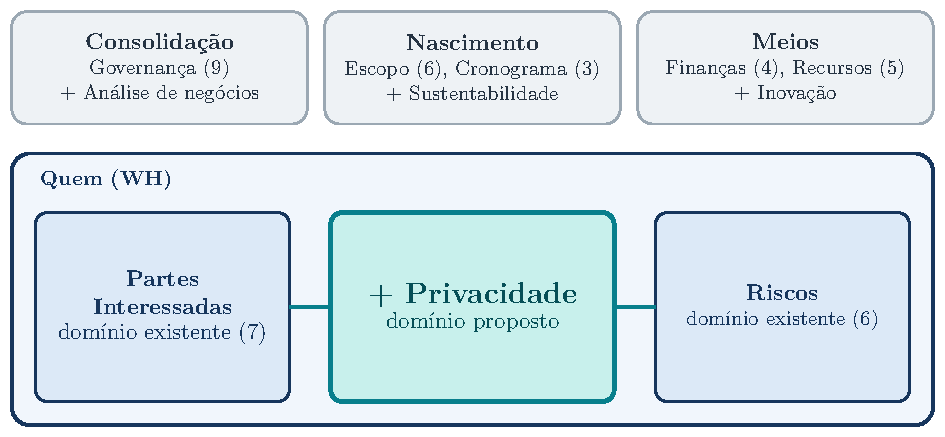
\includegraphics[width=\linewidth]{out/Fig1_PT.pdf}
\caption{Posição do domínio proposto entre as concentrações.}
\end{figure}

As quatro concentrações são a organização adotada neste trabalho. \textbf{Privacidade} é a contribuição do grupo à concentração \textbf{Quem}.

\vspace{0.3cm}
\LHead{3. Aderência aos 6 princípios}

\textbf{1AHV} Visão integral do fluxo de dados\\
\textbf{2FOV} Benefício frente ao dano potencial\\
\textbf{3QPD} Privacidade como qualidade verificável\\
\textbf{4BAL} Decisões e responsáveis registrados\\
\textbf{5SPA} Efeitos duradouros sobre pessoas\\
\textbf{6BEC} Contestação e aprendizado

\vspace{0.3cm}
\LHead{4. Oito processos propostos: decisão e evidência}

{\small
\begin{itemize}
    \item \textbf{P1 Identificar titulares e dados} $\rightarrow$ inventário inicial.
    \item \textbf{P2 Definir finalidade e papéis} $\rightarrow$ plano de privacidade.
    \item \textbf{P3 Avaliar efeitos sobre pessoas} $\rightarrow$ avaliação; RIPD quando cabível.
    \item \textbf{P4 Escolher respostas proporcionais} $\rightarrow$ plano de controles.
    \item \textbf{P5 Informar e encaminhar pedidos} $\rightarrow$ registro de respostas.
    \item \textbf{P6 Aplicar controles e tratar incidentes} $\rightarrow$ evidências de execução.
    \item \textbf{P7 Revisar eficácia e novas finalidades} $\rightarrow$ revisão do plano.
    \item \textbf{P8 Decidir conservação, transferência ou eliminação} $\rightarrow$ registro de destino.
\end{itemize}
}

\end{textblock}

% ------------------------------- COLUNA DIREITA -------------------------------
\begin{textblock}{11}(12,2.0)

\LHead{5. Privacidade ao longo do projeto}

\begin{figure}[h!]
\centering
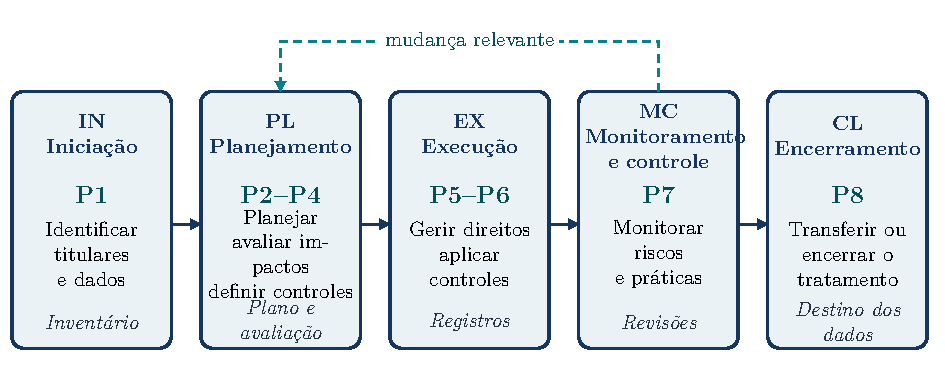
\includegraphics[width=\linewidth]{out/Fig2_PT.pdf}
\caption{Privacidade ao longo do projeto.}
\end{figure}

P1--P8 são \textbf{processos propostos pelo grupo}, distribuídos pelas cinco áreas de foco. A seta indica reavaliação; o tratamento de dados pode continuar após o encerramento.

\vspace{0.3cm}
\LHead{6. Gêmeos digitais e exposição de dados}

\begin{figure}[h!]
\centering
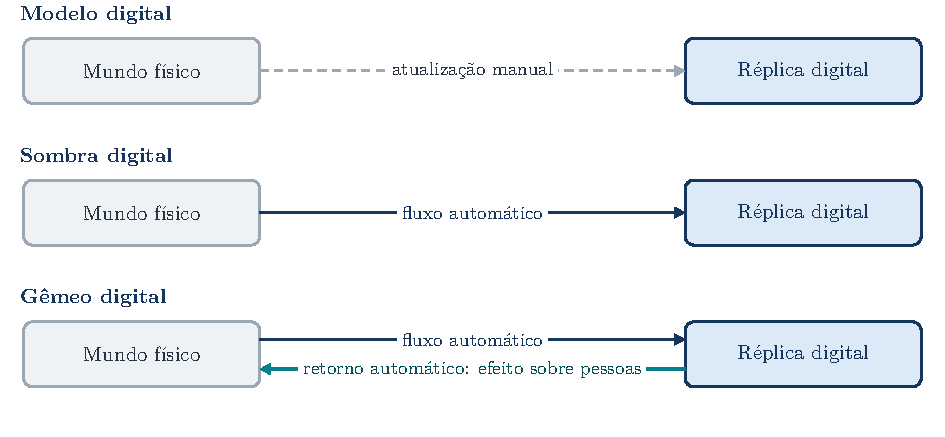
\includegraphics[width=\linewidth]{out/Fig4_PT.pdf}
\caption{Gêmeos digitais e exposição de dados.}
\end{figure}

A classificação segue Kritzinger et al. [11]. Fluxos automáticos e frequentes exigem atenção a titulares, finalidades, compartilhamentos, riscos e destino dos registros [17].

\vspace{0.3cm}
\LHead{7. Referências principais}

{\normalsize
[11] KRITZINGER, W. et al. Digital twin in manufacturing: a categorical literature review and classification. \textbf{IFAC-PapersOnLine}, v. 51, n. 11, 2018.

[13] PMI. \textbf{The Standard for Project Management and A Guide to the PMBOK (PMBOK Guide)}. 8. ed., 2025.

[17] WANG, Y. et al. A survey on digital twins: architecture, enabling technologies, security and privacy, and future prospects. \textbf{IEEE Internet of Things Journal}, v. 10, n. 17, 2023.

\textit{Numeração do relatório completo.}
% \textit{P1--P8 são uma proposta acadêmica e não integram oficialmente o PMBOK 8.}  % NOTA-COMENTADA
}

\end{textblock}

% AVISO-IA:INICIO
\begin{textblock}{23}(0,11.4)
{\small\noindent \textbf{Uso de IA:} IA generativa (ChatGPT Astral 6 Sol e Sonnet 5.5, modo alto) apoiou a revisão de texto, a formatação, a criação de figuras e a formulação de tabelas. O grupo é responsável pelo conteúdo (COPE, 2023: \texttt{publicationethics.org/guidance/cope-position/authorship-and-ai-tools}).\par}
\end{textblock}
% AVISO-IA:FIM

\end{document}
